\documentclass{article}

% Language setting
% Replace `english' with e.g. `spanish' to change the document language
\usepackage[spanish]{babel}

% Set page size and margins
% Replace `letterpaper' with`a4paper' for UK/EU standard size
\usepackage[a4paper,top=1cm,bottom=2cm,left=3cm,right=3cm,marginparwidth=1.75cm]{geometry}

% Useful packages
\usepackage{amsmath}
\usepackage{graphicx}
\usepackage[colorlinks=true, allcolors=blue]{hyperref}
\usepackage{listings}

\title{Ejercicio 1 Bloque II: Fundamentos de la radiocomunicación}
\author{André Yermak y Álvaro Hernández}

\begin{document}
\maketitle


\section{Realización de la gráfica}

\subsection{Planteamiento del problema}

Para la realización de la gráfica, se necesita primero entender lo que se pide en el enunciado. Se plantea un problema de diseño de redes inalámbricas basadas en el estandar 802.11g, en el entorno de una oficina. 
Se usará el modelo \verb|Path-Loss|, y mediante la fórmula de las pérdidas de propagación, se calculará el número máximo de paredes que pueda haber respecto a la distancia para poder recibir una velocidad de transmisión de 54 Mbps. 

Una vez planteado el enunciado, se analizan las variables de entrada necesarias según el enunciado:

\begin{itemize}
      \item \textbf{Potencia transmitida:} la variable potencia transmitida, no se proporciona en el enunciado, se asume como 100mW (20dBm) debido a la documentación del punto de acceso \textbf{Cisco Aironet 1200} y la regulación de potencia en España. 
      \item \textbf{Sensibilidad:} tampoco será proporcionada, en la misma documentaciónd del punto de acceso se indica la sensibilidad buscada, que en este caso será de -72dBm para una velocidad de 54 Mbps.
      \item \textbf{Atenuación de la pared:} según las diapositivas de la asignatura, será 6dB en interiores como oficinas.
      \item \textbf{$\alpha$ del modelo} \verb|Path-Loss|: proporcionada en el enunciado, el valor será de 1.8.
      \item  \textbf{Frecuencia:} es conocida la frecuencia en el estandar $802.11g$, que será de $2.4GHz$.
\end{itemize}
\subsection{Resolución teórica}

Una vez conocidos los valores de las variables de entrada, y que la distancia también es conocida, ya que se tomarán varios valores al estar en el eje de abcisas de nuestra gráfica, se puede volver a la fórmula:

$$L_{\text{PATHLOSS}} = \left(\frac{4\pi}{\lambda}\right)^{2}d^\alpha$$

Donde $L$ es $\frac{P_{TX}}{P_{RX}}$, y $\lambda$ será $\frac{f}{c}$, con $c$ como la velocidad de la luz $3 \cdot 10^8$. Se despejará el valor de la potencia recibida según las pérdidas de propagación.

$$\frac{P_{TX}}{P_{RX}} = \left(\frac{4\pi f}{c}\right)^2 d^\alpha \quad \rightarrow \quad P_{RX}  = \frac{P_{TX}}{\left(\frac{4\pi f}{c}\right)^2 d^\alpha }$$

Con la potencia recibida (en mW) según las pérdidas de propagación no será suficiente, pues existen paredes en la oficina. El objetivo será buscar el número máximo de paredes que puedan hacer posible la transmisión a 54 Mbps, por lo que, sabiendo que la sensibilidad es de -72 dBm, habrá que pasar la potencia recibida a dBm, y restando la atenuación de las paredes se podrá obtener una $P_{RX}'$ para comparar con los $-72dBm$. 

$$P_{RX}' (dBm) = P_{RX}(dBm) - N \cdot 6 dB \geq -72dBm$$ 

\quad

Por lo que existirá un número N máximo de paredes que se pueda atravesar respecto a la distancia introducida en la fórmula anteriormente. Para despejarlo, valdrá con igualarlo como una ecuación común y, al ser las paredes un número entero, redondearlo a la baja.



\subsection{Cálculos en excel y procesamiento de la gráfica}

Una vez resuelto teóricamente el problema, en el excel presentado, se usarán las filas y columnas necesarias para los valores de entrada, en este caso la columna $C$ contendrá los valores necesarios para la resolución de la fórmula.

\begin{figure}[h]
      \centering
      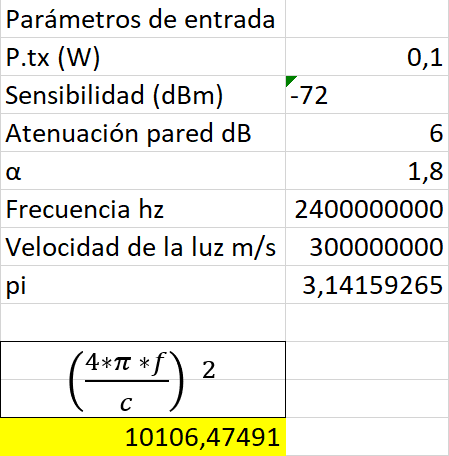
\includegraphics[width=0.35\linewidth]{exceldatos.png}
      \caption{\label{fig:excele} Parámetros de entrada en el excel.}
\end{figure}

Como la distancia estará en la gráfica, se necesitarán varios valores. (ver archivo xlsx).
Para cada valor, se calculará la $P_{RX}$ con la fórmula despejada anteriormente, y en otra fila, se obtiene la $P_{RX}$ en dBm.

Una vez obtenidas las potencias para las distintas distancias, se puede observar cuál será el valor de N paredes que hacen que la $P_{RX}'$ tenga el valor de la sensibilidad. Finalmente, se redondeará a la baja, y se tomará en el eje de cordenadas; En el eje de abcisas estará la fila con los valores usados en la distancia.

\begin{figure}[h]
      \centering
      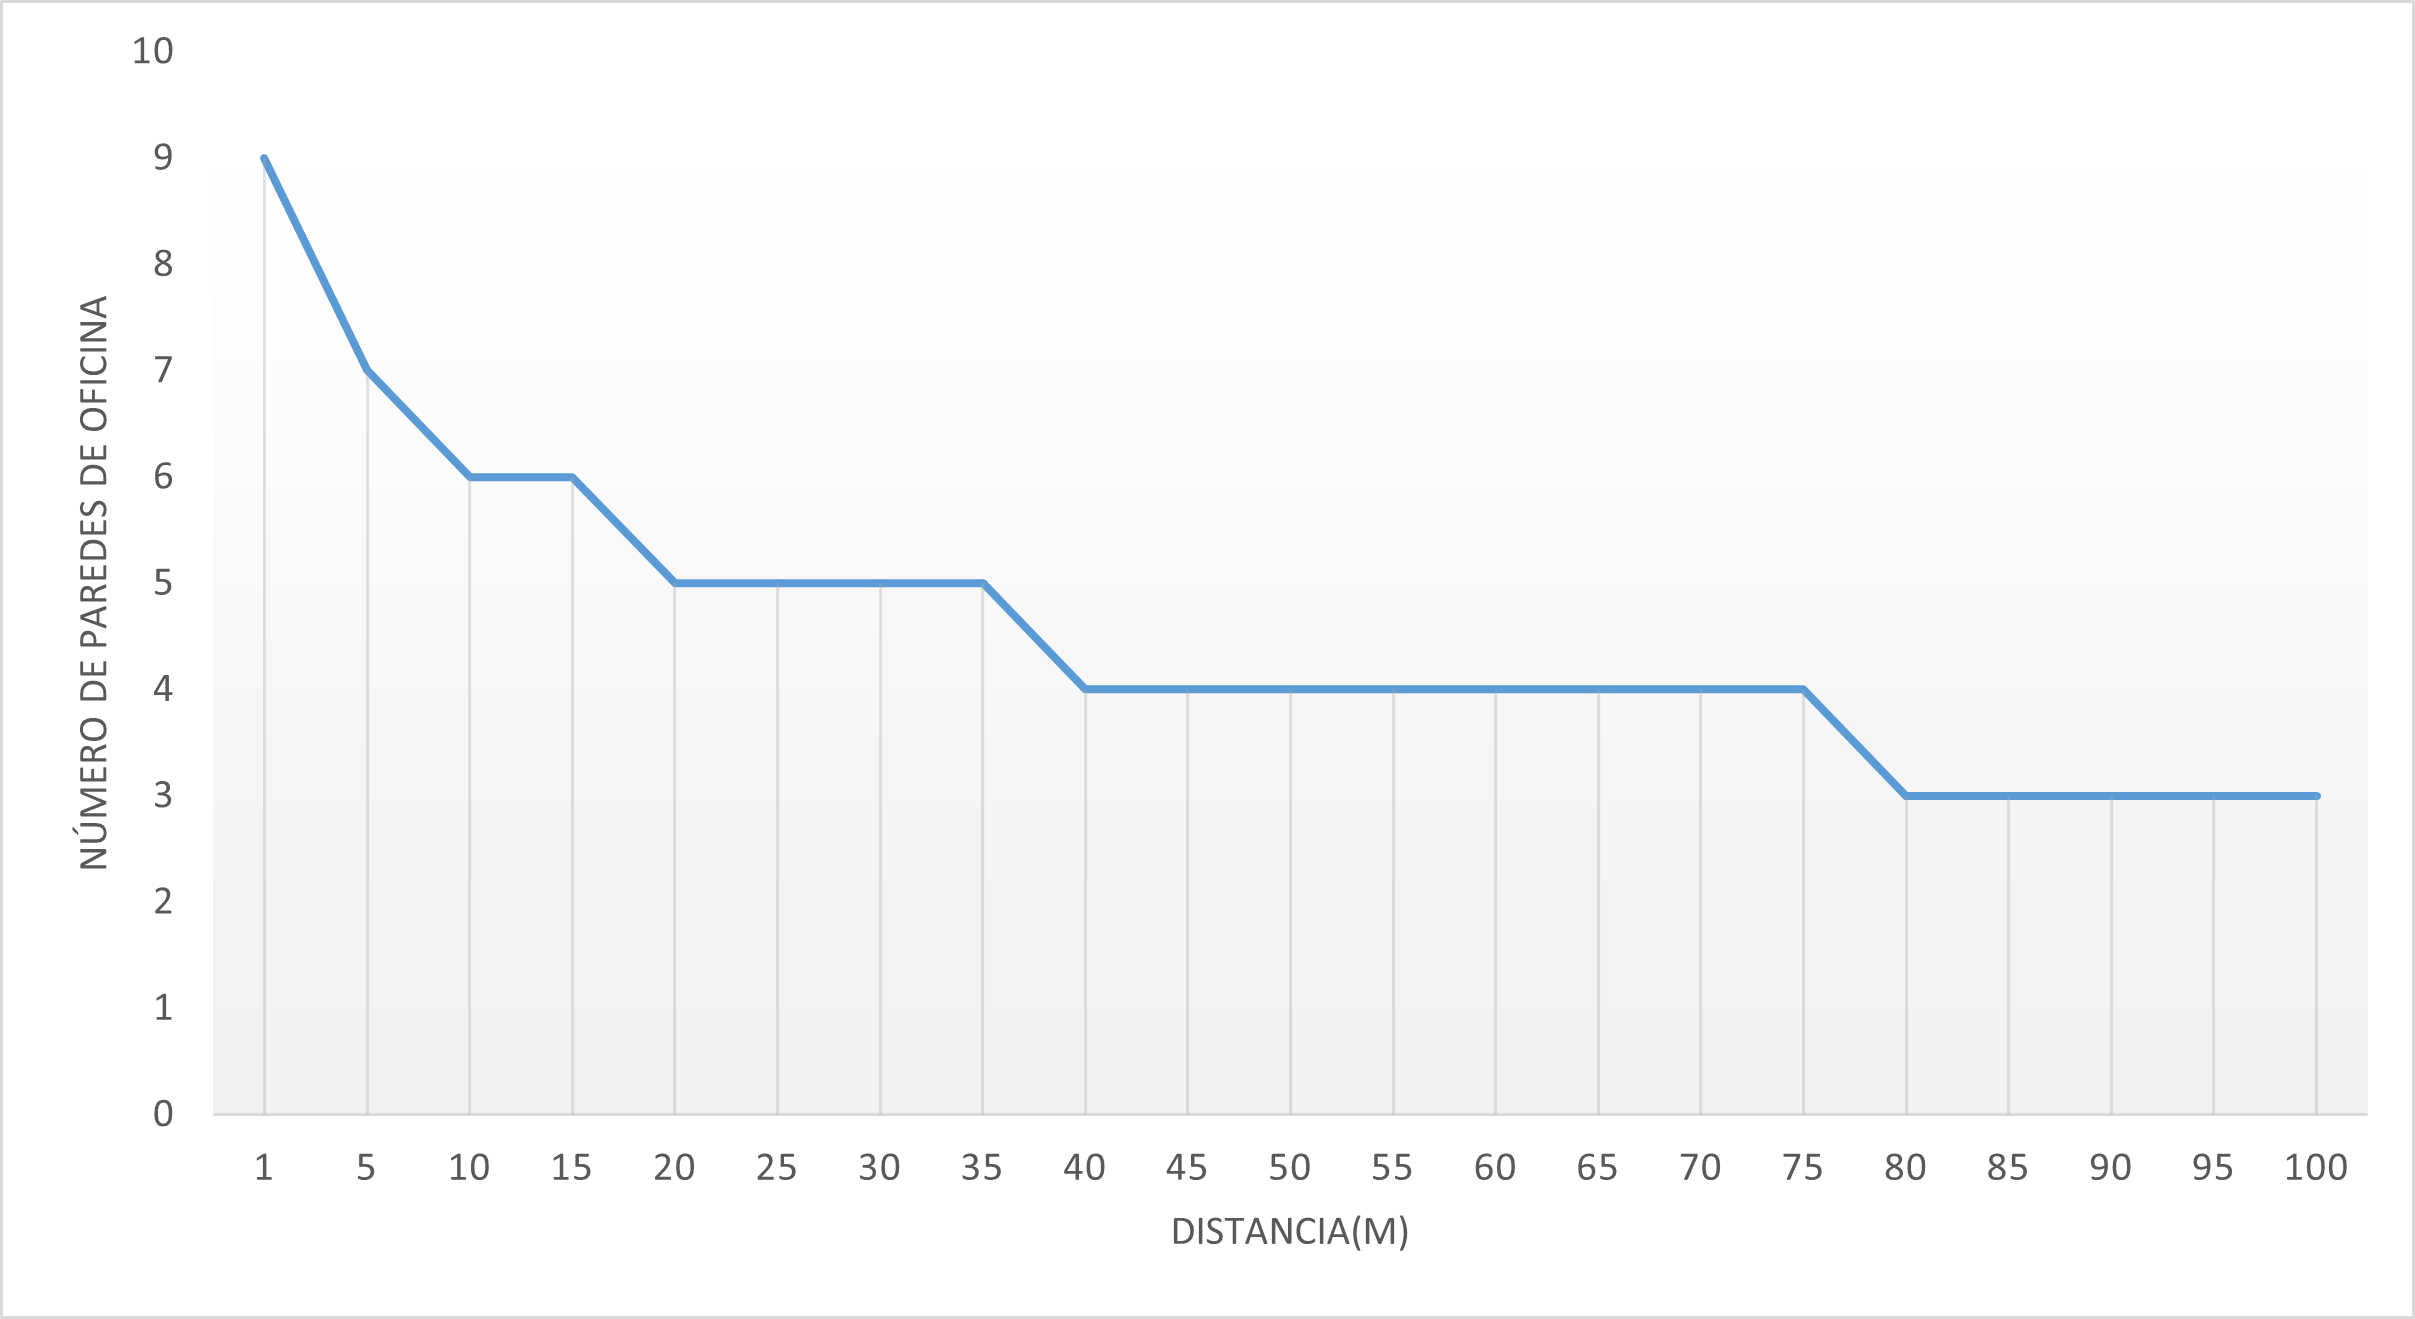
\includegraphics[width=0.6\linewidth]{grafica paredes.png}
      \caption{\label{fig:grafic} Gráfica obtenida.}
\end{figure}

\newpage

\section{Preguntas sobre la gráfica}

\textbf{¿Es posible realizar una transmisión a una distancia de 20 metros cuando entre transmisor y
receptor hay 5 paredes?}



No. Viendo la gráfica obtenida en Excel, no se logra una transmisión satisfactoria con este escenario. 

\quad

\textbf{Desde un punto de vista teórico justifique cómo podría realizarse la transmisión anterior.}

Siguiento la fórmula $P_{TX}(dBm)-L_{PATHLOSS}(dBm)- N \cdot L_{pared}(dB)=P_{RX}'(dBm)$, mientras que la potencia recibida sea mayor a la sensibilidad (-72 dBm en nuestro caso) la transmisión se hubiera realizado con éxito teóricamente. Con los datos obtenidos de Excel obtendríamos una potencia recibida de : $P_{RX}(dBm)=-73,46 dBm\leq -72 dBm$ \\ Por lo que la potencia recibida es menor, y no cumple el requisito.

\quad

\textbf{Desde un punto de vista práctico justifique si la transmisión podría realizarse.}

En la práctica basta con ver que un dispositivo no está recibiendo la velocidad solicitada de 54 Mbps sino a otra inferior.

\quad

\textbf{Justifique por qué en el modelo de Path Loss $\alpha$ es inferior a 2.}

El resultado de $\alpha$=1.8 se estima a que es una constante obtenida de interiores. Al existir obstáculos donde la onda pueda rebotar siempre hará que $\alpha$ sea mayor que 1 y perderá más potencia que en un camino ideal (por ejemplo el vacío), pero al no ser exterior, donde puede rebotar la señal en edificios, árboles, vehículos, $\alpha$ no llega a 3 o más como suele usarse en ese tipo de áreas urbanas.

\end{document}